\addchapheadtotoc

\chapter{Procedures}

The Gross-Pitaevskii equation is simulated using Python using a spatial finite difference method and the Runge-Kutta method for the time evolution. Numpy is used to discretize the wavefunction with matrices and the SciPy package is used to evolve the wavefunction through time. An initial wavefunction generated as a sinusoid independent of the lattice size and evolved prior to perturbation. This wavefunction is perturbed by superimposing a small sinusoid and both functions are allowed to evolve independently. The difference of these wavefunctions is recorded and a Lyapunov exponent can be calculated. 

\section{Numerical Derivatives}
For the spatial discretization, a 2D diagonal matrix was used to calculate the first derivative. To begin, recall the definition of a derivative, \begin{equation}
	f'(x) = \lim_{h \to 0} \frac{ f(x+h) - f(x) }{h} + O(h).
\end{equation}
To approximate the limit, we can take $h$ to be a small finite value relative to the target function $f(x)$. This equation is known as the \textit{forward difference}, as $h$ is \textit{forward} of $x$. In a similar fashion, the backward difference is given as \begin{equation}
	f'(x) = \lim_{h \to 0} \frac{f(x-h) - f(x)}{h} + O(h).
\end{equation}
Both the forward and backward differences can be averaged for a more accurate central difference approximation, \begin{equation}
	f'(x) = \lim_{h \to 0} \frac{f\left(x+\frac{h}{2}\right) - f\left(x - \frac{h}{2}\right)}{h} + O(h^2).
\end{equation}
For the second-order central difference approximation, it can be shown either directly or through the Taylor expansion \begin{equation}
	f''(x) = \lim_{h \to 0} \frac{f(x+h) - 2f(x) + f(x-h)}{h^2} + O(h^3).
\end{equation}
Note that this method has some truncation error due to the Taylor expansion. Additional higher-order terms $O(h^3)$ can be added for better precision at the expense of computational cost. 

\subsection{Matrix formulation}
In the second-order central difference approximation, each term at point $x$ depends on the previous and next spatial term. As the derivative operator is linear and many Python libraries support matrices including NumPy, we can convert the second-order derivative operator to a matrix. For a given function $f(x)$ discretized over $x$, the second derivative can be calculated using the matrices, \begin{align}
		\ket{f''(x)} & = \hat{D} \ket{f(x)} \notag \\
		\begin{pmatrix}
			f''(x_0) \\
			f''(x_1) \\
			f''(x_2) \\
			\vdots \\
			f''(x_{N-1})
		\end{pmatrix} & = \frac{1}{h^2}\begin{pmatrix}
			-2 & 1 & \\
			1 & -2 & 1 \\
			  & 1 & -2 & 1 \\
			  & & \ddots & \ddots & \ddots \\
			  & & & 1 & -2 & 1
	\end{pmatrix} \begin{pmatrix}
		f(x_0) \\
		f(x_1) \\
		f(x_2) \\
		\vdots \\
		f(x_{N-1})
	\end{pmatrix} \label{eq:mtxd2}.
	\end{align}
	For periodic boundary conditions, the first term of the derivative must wrap around and use the last term in the derivative calculation, and vice versa. This results in modifying \eqref{eq:mtxd2} to  \begin{align}
		\begin{pmatrix}
			f''(x_0) \\
			f''(x_1) \\
			f''(x_2) \\
			\vdots \\
			f''(x_{N-1})
		\end{pmatrix} & = \frac{1}{h^2}\begin{pmatrix}
			-2 & 1 & & & & 1\\
			1 & -2 & 1 \\
			& 1 & -2 & 1 \\
			& & \ddots & \ddots & \ddots \\
			1 & & & 1 & -2 & 1
		\end{pmatrix} \begin{pmatrix}
			f(x_0) \\
			f(x_1) \\
			f(x_2) \\
			\vdots \\
			f(x_{N-1})
		\end{pmatrix} \label{eq:mtxd2_periodic}.
	\end{align}
	From this matrix, the one-dimensional Laplacian term in the Gross-Pitaevskii equation can be approximated.
	
	\section{Gross-Pitaevskii equation and time evolution}
	From the second derivative matrix \eqref{eq:mtxd2_periodic}, the Python function in Listing \ref{lst:gpe} can be used to evolve the time-dependent Gross-Pitaevskii equation over time with \texttt{solve\_ivp} from the SciPy package. This function solves \eqref{eq:gpe} for $\pdv{\Psi}{t}$. Using this function definition, the Runge-Kutta method can be applied as an adaptive solver and the time evolution can be observed, resulting in a 2D matrix over time and space. Additionally, the relative and absolute tolerances can be lowered in the solver to ensure high precision.

	\begin{figure}[h]
		\begin{lstlisting}[language=Python, caption={The \texttt{solve\_ivp} wrapper function for the Gross-Pitaevskii equation. This function approximates \eqref{eq:gpe}.}, label={lst:gpe}]
	def compute_dpsi_dt(t, psi):
		""" Return dpsi/dt for the GPE. """
		phase = 1 / (1j * hbar * cooling_phase / np.abs(cooling_phase))
		n = abs(psi)**2
		return phase * (-hbar / 2 / m * (D2 @ psi) + (V(x) + g * n) * psi)
		\end{lstlisting}
	\end{figure}

	\section{Initial many-body wavefunction}
	Before perturbing the wavefunction when calculating the Lyapunov exponent, an initial wavefunction must be generated. Here, a function was used to generate sinusoidal noise with perioidic boundary conditions. This function generates an initial state independent of the dimensions of the lattice spacing. This function is shown in Listing \ref{lst:fouriernoise}.

	\section{Lyapunov exponent calculation}
	To calculate the Lyapunov exponent of the Gross-Pitaevskii equation, first we must generate a wavefunction and a perturbed copy, then evolve both through time and calculate the difference in Hilbert space. The Lyapunov exponent must be approximated, as the limits are not feasible as the time and spatial components are finite and discrete. Here, we will use an analog to the Lyapunov exponent by evolving the system until the distance is maximized and plateaued, as shown in Figure \ref{fig:lorenzexp}.
	
	An initial wavefunction is generated using Listing \ref{lst:fouriernoise}. A perturbed wavefunction is created by superimposing a small-amplitude sinusoid on the initial function. Both functions are evolved independently and the difference in wavefunctions are calculated over time using \eqref{eq:dist}. After a set time, the perturbed wavefunction is ``pulled back'' so the two wavefunctions meet, shown in Figure \ref{fig:pullbacks}. This process is repeated several times to ensure a maximal exponent can be found. The Lyapunov exponent is calculated for each iteration by taking a exponential fit of the differences as a function of time in the direction of the maximal Lyapunov exponent. 


	\begin{figure}[p]
		\centering
		 \begin{subfigure}[b]{0.75\textwidth}
			\centering
			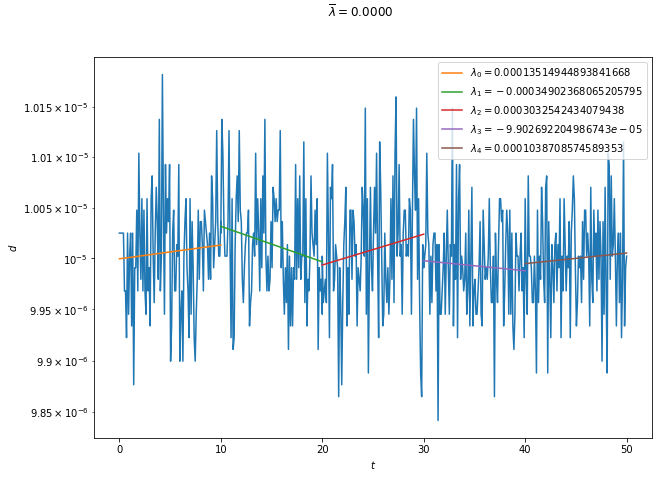
\includegraphics[width=\linewidth]{chapter3/pullbacks0}
			\caption{$g=0$}
			\label{fig:pullbacks0}
		\end{subfigure}
		
			\vspace{2em}
			
		 \begin{subfigure}[b]{0.75\textwidth}
			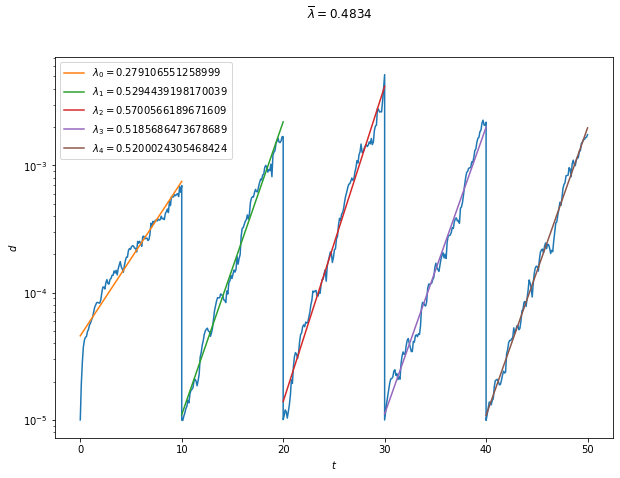
\includegraphics[width=\linewidth]{chapter3/pullbacks}
			\caption{$g=10$}
		\end{subfigure}
		\caption[An example of pulling back the perturbed wavefunction.]{An example of pulling back the perturbed wavefunction for two cases: the normal Schr\"odinger equation and the nonlinear case. }
		\label{fig:pullbacks}
	\end{figure}
	

	To ensure numerical error is minimized, after evolving the wavefunction through time, the wavefunction is evolved backwards through time. The difference between the original wavefunction and the reverse-time-evolved function must be within a small tolerance to ensure accuracy.
	
	Additionally, for the $g=0$ case, the Gross-Pitaevskii equation is the regular Schr\"odinger equation. This case is linear and should give no chaotic motion, and we should expect a zero Lyapunov exponent.
	
	\section{Experimental values}
	In the simulation, we set $\hbar=1$ and mass $m=1$. The periodic lattice is set to a length of $L=10$ length units, divided into 400 segments. The maximum time step size is set to $\Delta t = 0.01$ time units in the RK45 solver.	The units of time are \begin{align*}
		[t] & = \frac{[L]^2}{10^2} \frac{[m]}{[\hbar]}.
		\end{align*}
	The perturbation amplitude is set to \num{e-5} length units. When varying $g$, the system is allowed to evolve for 1 time unit with 100 steps. This process is repeated 5 times per $g$ value.
%	TODO: write out the units. 
%	
%	the time unit can be determined with \begin{align*}
%			t & = m L^2 / \hbar?
%		\end{align*}
%	How to go about finding what the time units are in SI units?
%	
%	Units of $g$?
	